%!TEX root = ../tfe.tex
\section{Test case to assess the implementation of the overturner model}
This note is an adaptation of \textit{Eric Deleersnijder}'s working paper \cite{deleersnijder2011test}.

%----------------------------------GOVERNING EQUATIONS--------------------------------------------------------%
\subsection{Governing equations}
Let us consider a water domain, whose width is denoted $B(t,\b{x})$, where $t$ is the time and $\b{x} = (y,z)$ is the position vector. The continuity equation is
\begin{equation} \label{eq:testcase:continuity}
	\frac{\partial B}{\partial t} + \nabla \cdot (B\b{u}) = 0,
\end{equation}
where $\b{u}(t,\b{x})$ is the latitudinally-averaged meridional velocity. Assuming that mixing along the parallels is sufficiently efficient, we may study the concentration of a passive tracer by means of a two-dimensional model. The latitudinally-averaged concentration of the tracer $C(t,\b{x})$ obeys the following partial differential equation :
\begin{equation} \label{eq:testcase:conservative}
	\frac{\partial (BC)}{\partial t} + \nabla \cdot (B \b{u} C) = Q\delta(\b{x} - \b{x}_1) + \nabla \cdot (B\b{K} \cdot \nabla C), 
\end{equation}
where $\b{K}$ is the diffusivity tensor (symmetric and positive definite); $\delta$ is the Dirac delta function with $\delta(\b{x}-\b{x}_n) = \delta(x-x_n)\delta(y-y_n)$; $Q(t)$ is the rate of release of a lineic source of length $B$ along the latitude direction located at $\b{x} = \b{x}_1$. If $C(t,\b x)$ represents the 
density of the tracer in water, then $Q(t)$ is the mass of tracer released per second by the source.

Equation \eqref{eq:testcase:conservative} is the so-called conservative form of the model. The convective form is obtained by combining equations \eqref{eq:testcase:continuity} and \eqref{eq:testcase:conservative}:
\begin{equation}  \label{eq:testcase:convective}
	\frac{\partial C}{\partial t} + \b{u} \cdot \nabla C = \frac{Q}{B} \delta(\b{x} - \b{x}_1) + \frac{1}{B} \nabla \cdot (B\b{K} \cdot \nabla C).
\end{equation}

%----------------------------------AN IDEALISED MODEL----------------------------------------------------------------------%
\subsection{An idealised model}
For our test case to be interesting, we must be able to compute its analytical solution. Accordingly, we make some simplifying assumptions which will allow us to compute the solution analytically.
First, we assume a constant width $B$ and a constant velocity field
\begin{equation} \label{eq:testcase:velocity}
	\b{u}(t,\b{x}) = v \b e_y + w \b e_z,
\end{equation}
where $\b e_y$ and $\b e_z$ are the unit vectors associated respectively with the $y$- and $z$-coordinate axis. Furthermore, the diffusivity tensor is supposed constant and diagonal :
\begin{equation} \label{eq:testcase:diffusivity}
	\b{K} = \begin{pmatrix}
			K_{yy} & 0 \\
			0 & K_{zz}
			\end{pmatrix},
\end{equation}
where $K_{yy},\ K_{zz} > 0$. Finally, we consider a sudden pointwise release of tracer at $t=0$. Hence, $Q(t)$ is of the form :
\begin{equation}
	Q(t) = M\delta(t),
\end{equation} 
where $M$ is the mass of tracer released at $t=0$.

Under these assumptions, equation \eqref{eq:testcase:convective} simplifies to :
\begin{equation} \label{eq:testcase}
	\frac{\partial C}{\partial t} + v \frac{\partial C}{\partial y} + w \frac{\partial C}{\partial z} = J \delta(t) \delta(y - y_1)\delta(z-z_1) + K_{yy} \frac{\partial^2 C}{\partial y^2} + K_{zz} \frac{\partial^2 C}{\partial z^2},
\end{equation}
where $J := M/B$.
For the sake of simplicity, we can forget about the fact that our model is width-integrated and consider that it is a purely two-dimensional model with a point-source
\begin{equation}
	Q := J\delta(t).
\end{equation}
A part of the physical meaning of the model is lost but this makes representations of the problem easier. $C$ now represents the two-dimensional density (i.e., in [$kg/m^2$]) of the tracer in water. $J$ can then be regarded as the mass of tracer released by the sudden point source at $\b x = \b x_1$. The three- and two-dimensional interpretations of the problem are represented on figure \ref{fig:testcase_scheme}.
% \footnote{This could be a bit confusing. As we switch from a 3-dimensional interpretation of the model to a 2-dimensional one, the meaning of the parameters changes. Hence, in the 3-dimensional interpretation, $C$ represents a 3D density ([$kg/m^3$]) and $M$ is a mass, whereas in the 2-dimensional interpretation, $C$ is a 2D density ([$kg/m^2$]) and $M$ has units of [$kg\,m$]. A part of the physical meaning of the model is lost, but this makes representations of the problem much easier.} \textcolor{red}{On peut aussi simplement considérer B = 1. Attention, si on opte finalement pour cette option, un facteur B doit être présent pour le calcul de certains diagnostiques.}
\begin{figure}[H]
	\centering
	\scalebox{.8}{% This file was created by matlab2tikz.
%
%The latest updates can be retrieved from
%  http://www.mathworks.com/matlabcentral/fileexchange/22022-matlab2tikz-matlab2tikz
%where you can also make suggestions and rate matlab2tikz.
%
\begin{tikzpicture}

\begin{axis}[%
width=0.307\textwidth,
height=0.333\textwidth,
at={(0\textwidth,0\textwidth)},
scale only axis,
plot box ratio=1 1 1,
xmin=0,
xmax=1,
xtick={0,1},
xticklabels={{0},{$B$}},
tick align=outside,
xlabel style={font=\color{white!15!black}},
xlabel={$x$},
ymin=0,
ymax=1,
ytick={0.3},
yticklabels={{$y_0$}},
ylabel style={font=\color{white!15!black}},
ylabel={$y$},
zmin=0,
zmax=1,
ztick={0.7},
zticklabels={{$z_0$}},
zlabel style={font=\color{white!15!black}},
zlabel={$z$},
view={69.6}{-21.2},
axis background/.style={fill=white}
]
\addplot3 [color=black, dotted]
 table[row sep=crcr] {%
0	0.3	0\\
0	0.3	0.00707070707070707\\
0	0.3	0.0141414141414141\\
0	0.3	0.0212121212121212\\
0	0.3	0.0282828282828283\\
0	0.3	0.0353535353535354\\
0	0.3	0.0424242424242424\\
0	0.3	0.0494949494949495\\
0	0.3	0.0565656565656566\\
0	0.3	0.0636363636363636\\
0	0.3	0.0707070707070707\\
0	0.3	0.0777777777777778\\
0	0.3	0.0848484848484848\\
0	0.3	0.0919191919191919\\
0	0.3	0.098989898989899\\
0	0.3	0.106060606060606\\
0	0.3	0.113131313131313\\
0	0.3	0.12020202020202\\
0	0.3	0.127272727272727\\
0	0.3	0.134343434343434\\
0	0.3	0.141414141414141\\
0	0.3	0.148484848484848\\
0	0.3	0.155555555555556\\
0	0.3	0.162626262626263\\
0	0.3	0.16969696969697\\
0	0.3	0.176767676767677\\
0	0.3	0.183838383838384\\
0	0.3	0.190909090909091\\
0	0.3	0.197979797979798\\
0	0.3	0.205050505050505\\
0	0.3	0.212121212121212\\
0	0.3	0.219191919191919\\
0	0.3	0.226262626262626\\
0	0.3	0.233333333333333\\
0	0.3	0.24040404040404\\
0	0.3	0.247474747474747\\
0	0.3	0.254545454545455\\
0	0.3	0.261616161616162\\
0	0.3	0.268686868686869\\
0	0.3	0.275757575757576\\
0	0.3	0.282828282828283\\
0	0.3	0.28989898989899\\
0	0.3	0.296969696969697\\
0	0.3	0.304040404040404\\
0	0.3	0.311111111111111\\
0	0.3	0.318181818181818\\
0	0.3	0.325252525252525\\
0	0.3	0.332323232323232\\
0	0.3	0.339393939393939\\
0	0.3	0.346464646464646\\
0	0.3	0.353535353535354\\
0	0.3	0.360606060606061\\
0	0.3	0.367676767676768\\
0	0.3	0.374747474747475\\
0	0.3	0.381818181818182\\
0	0.3	0.388888888888889\\
0	0.3	0.395959595959596\\
0	0.3	0.403030303030303\\
0	0.3	0.41010101010101\\
0	0.3	0.417171717171717\\
0	0.3	0.424242424242424\\
0	0.3	0.431313131313131\\
0	0.3	0.438383838383838\\
0	0.3	0.445454545454545\\
0	0.3	0.452525252525252\\
0	0.3	0.45959595959596\\
0	0.3	0.466666666666667\\
0	0.3	0.473737373737374\\
0	0.3	0.480808080808081\\
0	0.3	0.487878787878788\\
0	0.3	0.494949494949495\\
0	0.3	0.502020202020202\\
0	0.3	0.509090909090909\\
0	0.3	0.516161616161616\\
0	0.3	0.523232323232323\\
0	0.3	0.53030303030303\\
0	0.3	0.537373737373737\\
0	0.3	0.544444444444444\\
0	0.3	0.551515151515151\\
0	0.3	0.558585858585859\\
0	0.3	0.565656565656566\\
0	0.3	0.572727272727273\\
0	0.3	0.57979797979798\\
0	0.3	0.586868686868687\\
0	0.3	0.593939393939394\\
0	0.3	0.601010101010101\\
0	0.3	0.608080808080808\\
0	0.3	0.615151515151515\\
0	0.3	0.622222222222222\\
0	0.3	0.629292929292929\\
0	0.3	0.636363636363636\\
0	0.3	0.643434343434343\\
0	0.3	0.65050505050505\\
0	0.3	0.657575757575757\\
0	0.3	0.664646464646465\\
0	0.3	0.671717171717172\\
0	0.3	0.678787878787879\\
0	0.3	0.685858585858586\\
0	0.3	0.692929292929293\\
0	0.3	0.7\\
};
 \addplot3 [color=black, dotted]
 table[row sep=crcr] {%
0	0	0.7\\
0	0.00303030303030303	0.7\\
0	0.00606060606060606	0.7\\
0	0.00909090909090909	0.7\\
0	0.0121212121212121	0.7\\
0	0.0151515151515152	0.7\\
0	0.0181818181818182	0.7\\
0	0.0212121212121212	0.7\\
0	0.0242424242424242	0.7\\
0	0.0272727272727273	0.7\\
0	0.0303030303030303	0.7\\
0	0.0333333333333333	0.7\\
0	0.0363636363636364	0.7\\
0	0.0393939393939394	0.7\\
0	0.0424242424242424	0.7\\
0	0.0454545454545455	0.7\\
0	0.0484848484848485	0.7\\
0	0.0515151515151515	0.7\\
0	0.0545454545454545	0.7\\
0	0.0575757575757576	0.7\\
0	0.0606060606060606	0.7\\
0	0.0636363636363636	0.7\\
0	0.0666666666666667	0.7\\
0	0.0696969696969697	0.7\\
0	0.0727272727272727	0.7\\
0	0.0757575757575758	0.7\\
0	0.0787878787878788	0.7\\
0	0.0818181818181818	0.7\\
0	0.0848484848484849	0.7\\
0	0.0878787878787879	0.7\\
0	0.0909090909090909	0.7\\
0	0.0939393939393939	0.7\\
0	0.096969696969697	0.7\\
0	0.1	0.7\\
0	0.103030303030303	0.7\\
0	0.106060606060606	0.7\\
0	0.109090909090909	0.7\\
0	0.112121212121212	0.7\\
0	0.115151515151515	0.7\\
0	0.118181818181818	0.7\\
0	0.121212121212121	0.7\\
0	0.124242424242424	0.7\\
0	0.127272727272727	0.7\\
0	0.13030303030303	0.7\\
0	0.133333333333333	0.7\\
0	0.136363636363636	0.7\\
0	0.139393939393939	0.7\\
0	0.142424242424242	0.7\\
0	0.145454545454545	0.7\\
0	0.148484848484848	0.7\\
0	0.151515151515152	0.7\\
0	0.154545454545455	0.7\\
0	0.157575757575758	0.7\\
0	0.160606060606061	0.7\\
0	0.163636363636364	0.7\\
0	0.166666666666667	0.7\\
0	0.16969696969697	0.7\\
0	0.172727272727273	0.7\\
0	0.175757575757576	0.7\\
0	0.178787878787879	0.7\\
0	0.181818181818182	0.7\\
0	0.184848484848485	0.7\\
0	0.187878787878788	0.7\\
0	0.190909090909091	0.7\\
0	0.193939393939394	0.7\\
0	0.196969696969697	0.7\\
0	0.2	0.7\\
0	0.203030303030303	0.7\\
0	0.206060606060606	0.7\\
0	0.209090909090909	0.7\\
0	0.212121212121212	0.7\\
0	0.215151515151515	0.7\\
0	0.218181818181818	0.7\\
0	0.221212121212121	0.7\\
0	0.224242424242424	0.7\\
0	0.227272727272727	0.7\\
0	0.23030303030303	0.7\\
0	0.233333333333333	0.7\\
0	0.236363636363636	0.7\\
0	0.239393939393939	0.7\\
0	0.242424242424242	0.7\\
0	0.245454545454545	0.7\\
0	0.248484848484848	0.7\\
0	0.251515151515152	0.7\\
0	0.254545454545455	0.7\\
0	0.257575757575758	0.7\\
0	0.260606060606061	0.7\\
0	0.263636363636364	0.7\\
0	0.266666666666667	0.7\\
0	0.26969696969697	0.7\\
0	0.272727272727273	0.7\\
0	0.275757575757576	0.7\\
0	0.278787878787879	0.7\\
0	0.281818181818182	0.7\\
0	0.284848484848485	0.7\\
0	0.287878787878788	0.7\\
0	0.290909090909091	0.7\\
0	0.293939393939394	0.7\\
0	0.296969696969697	0.7\\
0	0.3	0.7\\
};
 \addplot3 [color=black, dashed]
 table[row sep=crcr] {%
0	0.3	0.7\\
0.0101010101010101	0.3	0.7\\
0.0202020202020202	0.3	0.7\\
0.0303030303030303	0.3	0.7\\
0.0404040404040404	0.3	0.7\\
0.0505050505050505	0.3	0.7\\
0.0606060606060606	0.3	0.7\\
0.0707070707070707	0.3	0.7\\
0.0808080808080808	0.3	0.7\\
0.0909090909090909	0.3	0.7\\
0.101010101010101	0.3	0.7\\
0.111111111111111	0.3	0.7\\
0.121212121212121	0.3	0.7\\
0.131313131313131	0.3	0.7\\
0.141414141414141	0.3	0.7\\
0.151515151515152	0.3	0.7\\
0.161616161616162	0.3	0.7\\
0.171717171717172	0.3	0.7\\
0.181818181818182	0.3	0.7\\
0.191919191919192	0.3	0.7\\
0.202020202020202	0.3	0.7\\
0.212121212121212	0.3	0.7\\
0.222222222222222	0.3	0.7\\
0.232323232323232	0.3	0.7\\
0.242424242424242	0.3	0.7\\
0.252525252525253	0.3	0.7\\
0.262626262626263	0.3	0.7\\
0.272727272727273	0.3	0.7\\
0.282828282828283	0.3	0.7\\
0.292929292929293	0.3	0.7\\
0.303030303030303	0.3	0.7\\
0.313131313131313	0.3	0.7\\
0.323232323232323	0.3	0.7\\
0.333333333333333	0.3	0.7\\
0.343434343434343	0.3	0.7\\
0.353535353535354	0.3	0.7\\
0.363636363636364	0.3	0.7\\
0.373737373737374	0.3	0.7\\
0.383838383838384	0.3	0.7\\
0.393939393939394	0.3	0.7\\
0.404040404040404	0.3	0.7\\
0.414141414141414	0.3	0.7\\
0.424242424242424	0.3	0.7\\
0.434343434343434	0.3	0.7\\
0.444444444444444	0.3	0.7\\
0.454545454545455	0.3	0.7\\
0.464646464646465	0.3	0.7\\
0.474747474747475	0.3	0.7\\
0.484848484848485	0.3	0.7\\
0.494949494949495	0.3	0.7\\
0.505050505050505	0.3	0.7\\
0.515151515151515	0.3	0.7\\
0.525252525252525	0.3	0.7\\
0.535353535353535	0.3	0.7\\
0.545454545454545	0.3	0.7\\
0.555555555555556	0.3	0.7\\
0.565656565656566	0.3	0.7\\
0.575757575757576	0.3	0.7\\
0.585858585858586	0.3	0.7\\
0.595959595959596	0.3	0.7\\
0.606060606060606	0.3	0.7\\
0.616161616161616	0.3	0.7\\
0.626262626262626	0.3	0.7\\
0.636363636363636	0.3	0.7\\
0.646464646464647	0.3	0.7\\
0.656565656565657	0.3	0.7\\
0.666666666666667	0.3	0.7\\
0.676767676767677	0.3	0.7\\
0.686868686868687	0.3	0.7\\
0.696969696969697	0.3	0.7\\
0.707070707070707	0.3	0.7\\
0.717171717171717	0.3	0.7\\
0.727272727272727	0.3	0.7\\
0.737373737373737	0.3	0.7\\
0.747474747474748	0.3	0.7\\
0.757575757575758	0.3	0.7\\
0.767676767676768	0.3	0.7\\
0.777777777777778	0.3	0.7\\
0.787878787878788	0.3	0.7\\
0.797979797979798	0.3	0.7\\
0.808080808080808	0.3	0.7\\
0.818181818181818	0.3	0.7\\
0.828282828282828	0.3	0.7\\
0.838383838383838	0.3	0.7\\
0.848484848484849	0.3	0.7\\
0.858585858585859	0.3	0.7\\
0.868686868686869	0.3	0.7\\
0.878787878787879	0.3	0.7\\
0.888888888888889	0.3	0.7\\
0.898989898989899	0.3	0.7\\
0.909090909090909	0.3	0.7\\
0.919191919191919	0.3	0.7\\
0.929292929292929	0.3	0.7\\
0.939393939393939	0.3	0.7\\
0.94949494949495	0.3	0.7\\
0.95959595959596	0.3	0.7\\
0.96969696969697	0.3	0.7\\
0.97979797979798	0.3	0.7\\
0.98989898989899	0.3	0.7\\
1	0.3	0.7\\
};
 \addplot3 [color=black, draw=none, mark size=2.5pt, mark=*, mark options={solid, black}]
 table[row sep=crcr] {%
0	0.3	0.7\\
};
 \addplot3 [color=black, draw=none, mark size=2.5pt, mark=*, mark options={solid, black}]
 table[row sep=crcr] {%
1	0.3	0.7\\
};
 \end{axis}

\begin{axis}[%
width=0.552\textwidth,
height=0.409\textwidth,
at={(-0.132\textwidth,-0.045\textwidth)},
scale only axis,
xmin=0,
xmax=1,
ymin=0,
ymax=1,
axis line style={draw=none},
ticks=none,
axis x line*=bottom,
axis y line*=left
]
\node[below right, align=left]
at (rel axis cs:0.4,0.63) {$Q$};
\addplot [color=black, dashed, forget plot]
  table[row sep=crcr]{%
0.646191646191646	0.654058043117745\\
0.718673218673219	0.64179104477612\\
};
\addplot [color=black, dashed, forget plot]
  table[row sep=crcr]{%
0.793611793611793	0.85140464344942\\
0.866093366093366	0.839137645107795\\
};
\addplot [color=black, dashed, forget plot]
  table[row sep=crcr]{%
0.796068796068795	0.307457711442787\\
0.868550368550368	0.295190713101162\\
};
\addplot [color=black, dashed, forget plot]
  table[row sep=crcr]{%
0.648648648648648	0.108452736318409\\
0.721130221130221	0.0961857379767835\\
};
\addplot [color=black, dashed, forget plot]
  table[row sep=crcr]{%
0.313267813267813	0.935981757877281\\
0.385749385749385	0.923714759535655\\
};
\addplot [color=black, dashed, forget plot]
  table[row sep=crcr]{%
0.164619164619164	0.740293532338309\\
0.237100737100737	0.728026533996684\\
};
\addplot [color=black, dashed, forget plot]
  table[row sep=crcr]{%
0.168304668304668	0.196346600331676\\
0.24078624078624	0.18407960199005\\
};
\addplot [color=black, dashed, forget plot]
  table[row sep=crcr]{%
0.23955773955774	0.808286898839139\\
0.23955773955774	0.724709784411278\\
};
\addplot [color=black, dashed, forget plot]
  table[row sep=crcr]{%
0.39066339066339	1.00895024875622\\
0.39066339066339	0.92537313432836\\
};
\addplot [color=black, dashed, forget plot]
  table[row sep=crcr]{%
0.793611793611793	0.937640132669985\\
0.793611793611793	0.854063018242124\\
};
\addplot [color=black, dashed, forget plot]
  table[row sep=crcr]{%
0.643734643734643	0.74029353233831\\
0.643734643734643	0.656716417910449\\
};
\addplot [color=black, dashed, forget plot]
  table[row sep=crcr]{%
0.239557739557739	0.184737976782754\\
0.239557739557739	0.101160862354894\\
};
\addplot [color=black, dashed, forget plot]
  table[row sep=crcr]{%
0.644963144963145	0.105135986733003\\
0.644963144963145	0.0215588723051426\\
};
\addplot [color=black, dashed, forget plot]
  table[row sep=crcr]
	\scalebox{.8}{% This file was created by matlab2tikz.
%
%The latest updates can be retrieved from
%  http://www.mathworks.com/matlabcentral/fileexchange/22022-matlab2tikz-matlab2tikz
%where you can also make suggestions and rate matlab2tikz.
%
\begin{tikzpicture}

\begin{axis}[%
width=0.333\textwidth,
height=0.333\textwidth,
at={(0\textwidth,0\textwidth)},
scale only axis,
plot box ratio=1 1 1,
xmin=0,
xmax=1,
xtick={0,1},
xticklabels={{0},{$B$}},
xlabel style={font=\color{white!15!black}},
xlabel={$x$},
ymin=0,
ymax=1,
ytick={0.3},
yticklabels={{$y_0$}},
ylabel style={font=\color{white!15!black}},
ylabel={$y$},
zmin=0,
zmax=1,
ztick={0.7},
zticklabels={{$z_0$}},
zlabel style={font=\color{white!15!black}},
zlabel={$z$},
view={90}{0},
axis background/.style={fill=white}
]
\addplot3 [color=black, dotted]
 table[row sep=crcr] {%
0	0.3	0\\
0	0.3	0.00707070707070707\\
0	0.3	0.0141414141414141\\
0	0.3	0.0212121212121212\\
0	0.3	0.0282828282828283\\
0	0.3	0.0353535353535354\\
0	0.3	0.0424242424242424\\
0	0.3	0.0494949494949495\\
0	0.3	0.0565656565656566\\
0	0.3	0.0636363636363636\\
0	0.3	0.0707070707070707\\
0	0.3	0.0777777777777778\\
0	0.3	0.0848484848484848\\
0	0.3	0.0919191919191919\\
0	0.3	0.098989898989899\\
0	0.3	0.106060606060606\\
0	0.3	0.113131313131313\\
0	0.3	0.12020202020202\\
0	0.3	0.127272727272727\\
0	0.3	0.134343434343434\\
0	0.3	0.141414141414141\\
0	0.3	0.148484848484848\\
0	0.3	0.155555555555556\\
0	0.3	0.162626262626263\\
0	0.3	0.16969696969697\\
0	0.3	0.176767676767677\\
0	0.3	0.183838383838384\\
0	0.3	0.190909090909091\\
0	0.3	0.197979797979798\\
0	0.3	0.205050505050505\\
0	0.3	0.212121212121212\\
0	0.3	0.219191919191919\\
0	0.3	0.226262626262626\\
0	0.3	0.233333333333333\\
0	0.3	0.24040404040404\\
0	0.3	0.247474747474747\\
0	0.3	0.254545454545455\\
0	0.3	0.261616161616162\\
0	0.3	0.268686868686869\\
0	0.3	0.275757575757576\\
0	0.3	0.282828282828283\\
0	0.3	0.28989898989899\\
0	0.3	0.296969696969697\\
0	0.3	0.304040404040404\\
0	0.3	0.311111111111111\\
0	0.3	0.318181818181818\\
0	0.3	0.325252525252525\\
0	0.3	0.332323232323232\\
0	0.3	0.339393939393939\\
0	0.3	0.346464646464646\\
0	0.3	0.353535353535354\\
0	0.3	0.360606060606061\\
0	0.3	0.367676767676768\\
0	0.3	0.374747474747475\\
0	0.3	0.381818181818182\\
0	0.3	0.388888888888889\\
0	0.3	0.395959595959596\\
0	0.3	0.403030303030303\\
0	0.3	0.41010101010101\\
0	0.3	0.417171717171717\\
0	0.3	0.424242424242424\\
0	0.3	0.431313131313131\\
0	0.3	0.438383838383838\\
0	0.3	0.445454545454545\\
0	0.3	0.452525252525252\\
0	0.3	0.45959595959596\\
0	0.3	0.466666666666667\\
0	0.3	0.473737373737374\\
0	0.3	0.480808080808081\\
0	0.3	0.487878787878788\\
0	0.3	0.494949494949495\\
0	0.3	0.502020202020202\\
0	0.3	0.509090909090909\\
0	0.3	0.516161616161616\\
0	0.3	0.523232323232323\\
0	0.3	0.53030303030303\\
0	0.3	0.537373737373737\\
0	0.3	0.544444444444444\\
0	0.3	0.551515151515151\\
0	0.3	0.558585858585859\\
0	0.3	0.565656565656566\\
0	0.3	0.572727272727273\\
0	0.3	0.57979797979798\\
0	0.3	0.586868686868687\\
0	0.3	0.593939393939394\\
0	0.3	0.601010101010101\\
0	0.3	0.608080808080808\\
0	0.3	0.615151515151515\\
0	0.3	0.622222222222222\\
0	0.3	0.629292929292929\\
0	0.3	0.636363636363636\\
0	0.3	0.643434343434343\\
0	0.3	0.65050505050505\\
0	0.3	0.657575757575757\\
0	0.3	0.664646464646465\\
0	0.3	0.671717171717172\\
0	0.3	0.678787878787879\\
0	0.3	0.685858585858586\\
0	0.3	0.692929292929293\\
0	0.3	0.7\\
};
 \addplot3 [color=black, dotted]
 table[row sep=crcr] {%
0	0	0.7\\
0	0.00303030303030303	0.7\\
0	0.00606060606060606	0.7\\
0	0.00909090909090909	0.7\\
0	0.0121212121212121	0.7\\
0	0.0151515151515152	0.7\\
0	0.0181818181818182	0.7\\
0	0.0212121212121212	0.7\\
0	0.0242424242424242	0.7\\
0	0.0272727272727273	0.7\\
0	0.0303030303030303	0.7\\
0	0.0333333333333333	0.7\\
0	0.0363636363636364	0.7\\
0	0.0393939393939394	0.7\\
0	0.0424242424242424	0.7\\
0	0.0454545454545455	0.7\\
0	0.0484848484848485	0.7\\
0	0.0515151515151515	0.7\\
0	0.0545454545454545	0.7\\
0	0.0575757575757576	0.7\\
0	0.0606060606060606	0.7\\
0	0.0636363636363636	0.7\\
0	0.0666666666666667	0.7\\
0	0.0696969696969697	0.7\\
0	0.0727272727272727	0.7\\
0	0.0757575757575758	0.7\\
0	0.0787878787878788	0.7\\
0	0.0818181818181818	0.7\\
0	0.0848484848484849	0.7\\
0	0.0878787878787879	0.7\\
0	0.0909090909090909	0.7\\
0	0.0939393939393939	0.7\\
0	0.096969696969697	0.7\\
0	0.1	0.7\\
0	0.103030303030303	0.7\\
0	0.106060606060606	0.7\\
0	0.109090909090909	0.7\\
0	0.112121212121212	0.7\\
0	0.115151515151515	0.7\\
0	0.118181818181818	0.7\\
0	0.121212121212121	0.7\\
0	0.124242424242424	0.7\\
0	0.127272727272727	0.7\\
0	0.13030303030303	0.7\\
0	0.133333333333333	0.7\\
0	0.136363636363636	0.7\\
0	0.139393939393939	0.7\\
0	0.142424242424242	0.7\\
0	0.145454545454545	0.7\\
0	0.148484848484848	0.7\\
0	0.151515151515152	0.7\\
0	0.154545454545455	0.7\\
0	0.157575757575758	0.7\\
0	0.160606060606061	0.7\\
0	0.163636363636364	0.7\\
0	0.166666666666667	0.7\\
0	0.16969696969697	0.7\\
0	0.172727272727273	0.7\\
0	0.175757575757576	0.7\\
0	0.178787878787879	0.7\\
0	0.181818181818182	0.7\\
0	0.184848484848485	0.7\\
0	0.187878787878788	0.7\\
0	0.190909090909091	0.7\\
0	0.193939393939394	0.7\\
0	0.196969696969697	0.7\\
0	0.2	0.7\\
0	0.203030303030303	0.7\\
0	0.206060606060606	0.7\\
0	0.209090909090909	0.7\\
0	0.212121212121212	0.7\\
0	0.215151515151515	0.7\\
0	0.218181818181818	0.7\\
0	0.221212121212121	0.7\\
0	0.224242424242424	0.7\\
0	0.227272727272727	0.7\\
0	0.23030303030303	0.7\\
0	0.233333333333333	0.7\\
0	0.236363636363636	0.7\\
0	0.239393939393939	0.7\\
0	0.242424242424242	0.7\\
0	0.245454545454545	0.7\\
0	0.248484848484848	0.7\\
0	0.251515151515152	0.7\\
0	0.254545454545455	0.7\\
0	0.257575757575758	0.7\\
0	0.260606060606061	0.7\\
0	0.263636363636364	0.7\\
0	0.266666666666667	0.7\\
0	0.26969696969697	0.7\\
0	0.272727272727273	0.7\\
0	0.275757575757576	0.7\\
0	0.278787878787879	0.7\\
0	0.281818181818182	0.7\\
0	0.284848484848485	0.7\\
0	0.287878787878788	0.7\\
0	0.290909090909091	0.7\\
0	0.293939393939394	0.7\\
0	0.296969696969697	0.7\\
0	0.3	0.7\\
};
 \addplot3 [color=black, dashed]
 table[row sep=crcr] {%
0	0.3	0.7\\
0.0101010101010101	0.3	0.7\\
0.0202020202020202	0.3	0.7\\
0.0303030303030303	0.3	0.7\\
0.0404040404040404	0.3	0.7\\
0.0505050505050505	0.3	0.7\\
0.0606060606060606	0.3	0.7\\
0.0707070707070707	0.3	0.7\\
0.0808080808080808	0.3	0.7\\
0.0909090909090909	0.3	0.7\\
0.101010101010101	0.3	0.7\\
0.111111111111111	0.3	0.7\\
0.121212121212121	0.3	0.7\\
0.131313131313131	0.3	0.7\\
0.141414141414141	0.3	0.7\\
0.151515151515152	0.3	0.7\\
0.161616161616162	0.3	0.7\\
0.171717171717172	0.3	0.7\\
0.181818181818182	0.3	0.7\\
0.191919191919192	0.3	0.7\\
0.202020202020202	0.3	0.7\\
0.212121212121212	0.3	0.7\\
0.222222222222222	0.3	0.7\\
0.232323232323232	0.3	0.7\\
0.242424242424242	0.3	0.7\\
0.252525252525253	0.3	0.7\\
0.262626262626263	0.3	0.7\\
0.272727272727273	0.3	0.7\\
0.282828282828283	0.3	0.7\\
0.292929292929293	0.3	0.7\\
0.303030303030303	0.3	0.7\\
0.313131313131313	0.3	0.7\\
0.323232323232323	0.3	0.7\\
0.333333333333333	0.3	0.7\\
0.343434343434343	0.3	0.7\\
0.353535353535354	0.3	0.7\\
0.363636363636364	0.3	0.7\\
0.373737373737374	0.3	0.7\\
0.383838383838384	0.3	0.7\\
0.393939393939394	0.3	0.7\\
0.404040404040404	0.3	0.7\\
0.414141414141414	0.3	0.7\\
0.424242424242424	0.3	0.7\\
0.434343434343434	0.3	0.7\\
0.444444444444444	0.3	0.7\\
0.454545454545455	0.3	0.7\\
0.464646464646465	0.3	0.7\\
0.474747474747475	0.3	0.7\\
0.484848484848485	0.3	0.7\\
0.494949494949495	0.3	0.7\\
0.505050505050505	0.3	0.7\\
0.515151515151515	0.3	0.7\\
0.525252525252525	0.3	0.7\\
0.535353535353535	0.3	0.7\\
0.545454545454545	0.3	0.7\\
0.555555555555556	0.3	0.7\\
0.565656565656566	0.3	0.7\\
0.575757575757576	0.3	0.7\\
0.585858585858586	0.3	0.7\\
0.595959595959596	0.3	0.7\\
0.606060606060606	0.3	0.7\\
0.616161616161616	0.3	0.7\\
0.626262626262626	0.3	0.7\\
0.636363636363636	0.3	0.7\\
0.646464646464647	0.3	0.7\\
0.656565656565657	0.3	0.7\\
0.666666666666667	0.3	0.7\\
0.676767676767677	0.3	0.7\\
0.686868686868687	0.3	0.7\\
0.696969696969697	0.3	0.7\\
0.707070707070707	0.3	0.7\\
0.717171717171717	0.3	0.7\\
0.727272727272727	0.3	0.7\\
0.737373737373737	0.3	0.7\\
0.747474747474748	0.3	0.7\\
0.757575757575758	0.3	0.7\\
0.767676767676768	0.3	0.7\\
0.777777777777778	0.3	0.7\\
0.787878787878788	0.3	0.7\\
0.797979797979798	0.3	0.7\\
0.808080808080808	0.3	0.7\\
0.818181818181818	0.3	0.7\\
0.828282828282828	0.3	0.7\\
0.838383838383838	0.3	0.7\\
0.848484848484849	0.3	0.7\\
0.858585858585859	0.3	0.7\\
0.868686868686869	0.3	0.7\\
0.878787878787879	0.3	0.7\\
0.888888888888889	0.3	0.7\\
0.898989898989899	0.3	0.7\\
0.909090909090909	0.3	0.7\\
0.919191919191919	0.3	0.7\\
0.929292929292929	0.3	0.7\\
0.939393939393939	0.3	0.7\\
0.94949494949495	0.3	0.7\\
0.95959595959596	0.3	0.7\\
0.96969696969697	0.3	0.7\\
0.97979797979798	0.3	0.7\\
0.98989898989899	0.3	0.7\\
1	0.3	0.7\\
};
 \addplot3 [color=black, draw=none, mark size=2.5pt, mark=*, mark options={solid, black}]
 table[row sep=crcr] {%
0	0.3	0.7\\
};
 \addplot3 [color=black, draw=none, mark size=2.5pt, mark=*, mark options={solid, black}]
 table[row sep=crcr] {%
1	0.3	0.7\\
};
 \end{axis}

\begin{axis}[%
width=0.563\textwidth,
height=0.417\textwidth,
at={(-0.125\textwidth,-0.053\textwidth)},
scale only axis,
xmin=0,
xmax=1,
ymin=0,
ymax=1,
axis line style={draw=none},
ticks=none,
axis x line*=bottom,
axis y line*=left
]
\node[below right, align=left]
at (rel axis cs:0.4,0.73) {$Q$};
\addplot [color=black, dashed, forget plot]
  table[row sep=crcr]{%
0.891891891891891	0.128353233830846\\
0.814496314496314	0.129353233830846\\
};
\addplot [color=black, dashed, forget plot]
  table[row sep=crcr]{%
0.889434889434889	0.922714759535655\\
0.812039312039311	0.923714759535655\\
};
\addplot [color=black, dashed, forget plot]
  table[row sep=crcr]{%
0.219901719901719	0.924373134328358\\
0.142506142506142	0.925373134328358\\
};
\addplot [color=black, dashed, forget plot]
  table[row sep=crcr]{%
0.218673218673218	0.128353233830846\\
0.141277641277641	0.129353233830846\\
};
\addplot [color=black, dashed, forget plot]
  table[row sep=crcr]{%
0.813267813267813	0.997341625207297\\
0.813267813267813	0.918739635157546\\
};
\addplot [color=black, dashed, forget plot]
  table[row sep=crcr]{%
0.813267813267813	0.12503648424544\\
0.813267813267813	0.0464344941956883\\
};
\addplot [color=black, dashed, forget plot]
  table[row sep=crcr]{%
0.222358722358722	0.123378109452737\\
0.222358722358722	0.0447761194029852\\
};
\addplot [color=black, dashed, forget plot]
  table[row sep=crcr]
	\caption{Illustration of the 3D and 2D interpretations of the model.}
    \label{fig:testcase_scheme}
\end{figure}


%------------------------------------PARAMETERS FOR TEST CASE 1--------------------------------------------------------------%
\subsubsection{Test case 1 : infinite domain}
The first (an most simple) test case is to consider an infinite domain, i.e.
\begin{equation} \label{eq:testcase:domain}
	-\infty < y,\, z < \infty,
\end{equation}
with nonzero velocities $v$ and $w$. This test case provides a check that our numerical implementation handles the diffusion and advection processes properly both in the $y$- and $z$-directions. The parameters are chosen from the values of the overturner model :
\begin{equation}
	v = \frac{\Psi}{H} = 4\e{-4}\mbox{ [$m/s$],}\quad  w = \frac{\Psi}{L}=1.33\e{-7}\mbox{ [$m/s$],}
\end{equation}
and
\begin{equation}
	K_{yy} = K_h = 10^{3} \mbox{ [$m^2/s$],}\quad K_{zz} = K_{v_{2}} = 10^{-4} \mbox{ [$m^2/s$].} 
\end{equation}
For the length scales of the overturner model, those diffusivities corresponds to Péclet numbers
\begin{equation}
	Pe_y = \frac{v}{K_{yy}/L} = 6,\quad Pe_z = \frac{w}{K_{zz}/H} = 6.67.
\end{equation}
Hence, in both the $y$- and $z$-directions, the transport is neither dominated by advection nor by diffusion. This is interesting as a test case since it allows to assess how the numerical solver handles both physical processes in both directions. 
Finally, $J = 50\,000$ particles are released at $t=0$ at the location $(y_1,z_1) = (0,0)$.

%------------------------------------PARAMETERS FOR TEST CASE 2--------------------------------------------------------------%
\subsubsection{Test case 2 : semi-infinite domain}
Another interesting case is to consider a semi-infinite domain with a wall at $z=0$ :
\begin{equation}
	-\infty < y < \infty,\quad 0 < z < \infty.
\end{equation}
This is useful to assess how our numerical model handles no-through boundary conditions. Again, the parameters values are related to the ones from the overturner model :
\begin{equation}
	v = \frac{\Psi}{H} = 4\e{-4}\mbox{ [$m/s$],}\quad  w = 0\mbox{ [$m/s$],}
\end{equation}
and
\begin{equation}
	K_{yy} = K_h = 10^{3} \mbox{ [$m^2/s$],}\quad K_{zz} = K_{v_{1}} = 10^{-1} \mbox{ [$m^2/s$].} 
\end{equation}
Notice the choice  of $K_{zz}$ : it is chosen equal to $K_{v_1}$, which is $10^3$ times larger than $K_{v_2}$, the value chosen for test case 1. The goal here is to assess that the boundary condition is well handled by the solver. Since $w=0$, only the vertical diffusivity could possibly drive the particles towards the wall. By increasing $K_{zz}$, we ensure that more particles will bounce against the wall, which is relevant in this context. $J = 50\,000$ particles are released at $t=0$ at the location $(y_1,z_1) = (0,H)$.



\subsection{Analytical solution and properties}
%------------------------------------------------Analytic GREEN's FUNCTION ---------------------------------------------%
\subsubsection{Green's function}
In order to build the analytical solution of the problem, we need to compute the Green's function associated to this particular problem. We derive the Green's function $G$ associated to test case 1. We will show later how this function can be used to compute the concentration for both test case 1 and test case 2. $\G$ is zero for $t<t'$ and is the solution of
\begin{equation} \label{eq:testcase_green}
	\begin{cases}
		\frac{\partial G}{\partial t} + v \frac{\partial G}{\partial y} + w\frac{\partial G}{\partial z} = K_{yy}\frac{\partial^2 G}{\partial y^2} + K_{zz}\frac{\partial^2 G}{\partial z^2}\\[.1cm]
		\left. G(t,t',y,z) \right \rvert_{t=t'} = \delta(y)\delta(z) 
	\end{cases}
\end{equation}
for $t \ge 0$, and on an infinite domain $\infty < y,\, z < \infty$. It can be shown that \textcolor{red}{source ? ou le papier de deleersnijder suffit ?}
\begin{equation} 
	G(t,t',y,z) = \frac{\exp\left[-\frac{(y-s_v)^2}{4K_{yy}\tau} -\frac{(z-s_w)^2}{4K_{zz}\tau} \right]}{4\pi\sqrt{K_{yy}K_{zz}}\tau},
\end{equation}
where $\tau = t-t'$ and 
\begin{equation}
	\b s(t,t') = (s_v(t,t'), s_w(t,t')) = \left(\int_{t'}^{t}v \rm d \xi, \int_{t'}^{t}w \rm d \xi \right) = \left(v\tau, w\tau\right).
\end{equation}

$G$ has some interesting properties. The "mass" of the solution is
\begin{equation} \label{eq:testcase:propmass}
	m(t,t') \equiv \int_{\R[2]} \G \rm d \b x = 1.
\end{equation}
The "center of mass" is located at
\begin{equation} \label{eq:testcase:propcenter}
	\b r(t,t') \equiv \frac{1}{m(t,t')} \int_{\R[2]} \b x \G \rm d \b x  = \b s(t,t').
\end{equation}
The variance of the solution is
\begin{equation} \label{eq:testcase:propvar}
	\sigma^2(t,t') \equiv \frac{1}{m(t,t')} \int_{\R[2]} \lvert \b x - \b r(t,t') \rvert^2 \G \rm d \b x = 2 (K_{yy}+K_{zz}) \tau.
\end{equation}

%------------------------------------------------Analytic TEST CASE 1 ---------------------------------------------%
\subsubsection{Test case 1}
The analytical solution of test case 1 is now obtained with the help of the Green's function derived above by computing the convolution between $G$ and the source terms :
\begin{align}
	C(t,\b x) &= \int_{0}^{t} \int_{\R[2]} G(t,t',\b x - \b x') J \delta(t) \delta(\b x- \b x_1) \rm d \b{x}' \rm dt'\nonumber\\
	&= J G(t,0,\b x - \b x_1).
\end{align}
The concentration profile for test case 1 is thus
\begin{equation}
	\frac{J}{4\pi\sqrt{K_{yy}K_{zz}}t}\exp\left[-\frac{(y-s_v)^2}{4K_{yy}t} -\frac{(z-s_w)^2}{4K_{zz}t} \right].
\end{equation}

The total mass of tracer present in the domain is
\begin{equation}
	m(t) \equiv \int_{\R[2]} C(t,\b x) \rm d \b x = J.
\end{equation}
Note that this number is independant of the transport processes.

The mass center is located at
\begin{align}
	\b r(t) &\equiv \frac{1}{m(t)} \int_{\R[2]} \b x C(t,\b x) \rm d \b x \nonumber \\
	&= \int_{\R[2]} \b x G(t,0,\b x - \b x_1) \rm d \b x \nonumber\\
	&= \int_{\R[2]} (\b x-\b x_1) G(t,0,\b x - \b x_1) + \b x_1 G(t,0,\b x - \b x_1) \rm d \b x\nonumber\\
	&= \b x_1 + \b s(t,0),
\end{align}
where properties \eqref{eq:testcase:propmass} and \eqref{eq:testcase:propcenter} are used to perform the last step.

Finally, the variance of the solution is
\begin{align}
	\sigma^2(t) &= \frac{1}{m(t)} \int_{\R[2]} \lvert \b x - \b r(t) \rvert^2 C(t,\b x) \rm d \b x \nonumber \\
	&= \int_{\R[2]} \lvert (\b x - \b x_1) - \b s(t,0)\rvert^2 G(t,0,\b x - \b x_1) \rm d \b x \nonumber \\
	&= 2(K_{yy}+K_{zz})t,
\end{align}
where property \eqref{eq:testcase:propvar} is used.

%------------------------------------------------Analytic TEST CASE 2 ---------------------------------------------%
\subsubsection{Test case 2}
To compute the solution to test case 2, a little trick must be applied. Consider the problem on an infinite domain with two sudden point sources of equal intensity located at $z = H$ and $z = -H$. By symmetry, one can see that the concentration of that problem in the region $[-\infty, \infty] \times [0, \infty]$ is precisely the concentration of test case 2. Hence, we can use the Green's function $G$ derived or test case 1 to compute the concentration. In this case, the convolution has to be performed with two point sources :
\begin{align}
	C(t,\b x) &= \int_{0}^{t} \int_{-\infty}^{\infty} \int_{-\infty}^{\infty} J \delta(t') \delta(y'- y_1)\left[\delta(z'-z_1)+\delta(z'+z_1)\right] G(t,t',y-y',z-z') \rm dy' \rm dz' \rm dt' \nonumber\\
	&= J \int_{0}^{t} \delta(t')[G(t,t',y-y_1,z-z_1)+G(t,t',y-y_1,z+z_1)] \label{tc2_eq2} \nonumber\\
	&= J[G(t,0,y-y_1,z-z_1)+G(t,0,y-y_1,z+z_1)].
\end{align}
The concentration of the tracer for test case 2 is thus
\begin{equation}
	C(t,y,z) = \frac{J}{4\pi\sqrt{K_{yy}K_{zz}}t}\exp\left[-\frac{(y-s_v)^2}{4K_{yy}t}\right]\left\{\exp\left[-\frac{(z-z_1)^2}{4K_{zz}t} \right] + \exp\left[-\frac{(z+z_1)^2}{4K_{zz}t} \right] \right\}
\end{equation}
The mass is obtained as
\begin{equation}
	m(t) \equiv \int_{0}^{\infty} \int_{-\infty}^{\infty} C(t,y,z) \rm dy \rm dz = J,
\end{equation}
i.e. the number of particles released at $t=0$. This result is obvious since there is no other source or sink, and we impose a no-through condition at the boundary.

\textcolor{blue}{NOTE : Le calcul du centre de masse me pose problème dans la direction z. On trouve assez facilement que $r_y = y_1 + s_v = y_1 + vt$. Par contre dans la direction z, il faut calculer $$\int_{0}^{\infty} z \left\{\exp\left[-\frac{(z-z_1)^2}{4K_{zz}t} \right] + \exp\left[-\frac{(z+z_1)^2}{4K_{zz}t} \right] \right\}\rm dz.$$ Pas sûr qu'une solution simple existe... Je m'attends à une expression du type "H + (...)", où (...) est un terme qui permet de tenir compte du décalage du centre de masse selon z à cause du rebond sur le mur, et qui serait donc une fonction de $K_{zz}$, $t$ et $z_1$.\\
Cependant, le calcul du centre de masse ne me parait pas indispensable et même si cela m'intrigue, j'ai du m'efforcer de lacher l'affaire pour ne pas passer la journée dessus. (D'autant plus que je peux les approximer numériquement à partir de l'expression analytique de la concentration.)}
% The mass center is
% \begin{align}
% 	\b r(t) &\equiv \frac{1}{m(t)} \int_{0}^{\infty} \int_{-\infty}^{\infty} (y \b e_y + z \b e_z) C(t,y,z) \rm dy \rm dz \nonumber \\
% 	&= \int_{0}^{\infty} \int_{-\infty}^{\infty} (y \b e_y + z \b e_z) \left[G(t,0,y-y_1,z-z_1)+G(t,0,y-y_1,z+z_1)\right] \rm dy \rm dz \nonumber\\
% 	&= \int_{\R[2]} (\b x-\b x_1) G(t,0,\b x - \b x_1) + \b x_1 G(t,0,\b x - \b x_1) \rm d \b x\nonumber\\
% 	&= \b x_1 + \b s(t,0),
% \end{align}

%-------------------------------------VALIDATION--------------------------------------------------------------------------------%
\section{Validation of the numerical solver}
This section aims to show that the numerical results obtained with the solver are in good agreement with the analytical ones. As the combination of the two test cases cover the main features of the overturner model, this constitutes a validation of the solver. 

Both test cases are simulated for 1 year with a time step of 1 hour, and $J = 50\,000$ \textcolor{red}{il faudrait tester avec $10\,000$} particles are released at $t=0$.
The concentration is computed at the final time $T = 1$ year on the domain $[y_{min},y_{max}] \times [z_{min},z_{max}]$, where the subscripts \textit{min} and \textit{max} stands for the minimal and maximal position at time $T$ amongst all the particles. The notation $C(y,z)$ will be used to denote $C(T,y,z)$ in the next. That domain is divided into $20 \times 20$ boxes, and the (normalized) concentration in a box is computed as the number of particles in that box divided by the total number of particles $J$.

%-------------------------------------RESULTS CASE 1----------------------------------------------------------------------------%
\subsection{Test case 1}
Figure \ref{fig:testcase_surf} shows a comparison between the numerical result and the analytical solution for the (normalized) concentrations. Dark (resp. light) shaded areas correspond to zones where the numerically computed concentration is "above" (resp. "below") the exact concentration. Figures \ref{fig:testcase_fixedy} and \ref{fig:testcase_fixedz} represent respectively a cut of the concentrations at fixed $y = r_{y,exact}$ and at fixed $z = r_{z,exact}$. The numerically computed concentration $C_{num}$ seems to be an appreciable approximation of the exact concentration $C_{exact}$. To be more specific, the maximal local error is 
\begin{equation}
	\|C_{exact}-C_{num}\|_{\infty} = 1.037\e{-3}.
\end{equation}
The centers of mass are located at
\begin{equation}
	\b r_{exact} = (12\,614.4,\,4.2) \mbox{ [$m$],}\quad \b r_{num} = (10\,985.3,\,4.4) \mbox{ [$m$]}.
\end{equation}
The relative error is
\begin{equation}
	\b e_r = \left \lvert \frac{\b r_{exact}-\b r_{num}}{\b r_{exact}} \right \rvert =  \left(1.29\e{-1}, 4.75\e{-2}\right),
\end{equation}
where the division is taken element-wise on the vectors. The 2-norm of the relative error is
\begin{equation}
	\| \b e_r \|_2 = 1.38\e{-1}.
\end{equation}
This can be seen as a quantification of the error on advection. To quantify the error on diffusion, we compute the variance of the concentration :
\begin{equation}
	\sigma^2_{exact} = 6.31\e{10} \mbox{ [$m^2$],}\quad \sigma^2_{num} = 6.35\e{10} \mbox{ [$m^2$].}
\end{equation}
The relative error is
\begin{equation}
	e_{\sigma^2} = \left \lvert \frac{\sigma^2_{exact}-\sigma^2_{num}}{\sigma^2_{exact}}\right \rvert = 7.26\e{-3}.
\end{equation}
\begin{figure}[H]
	\centering
	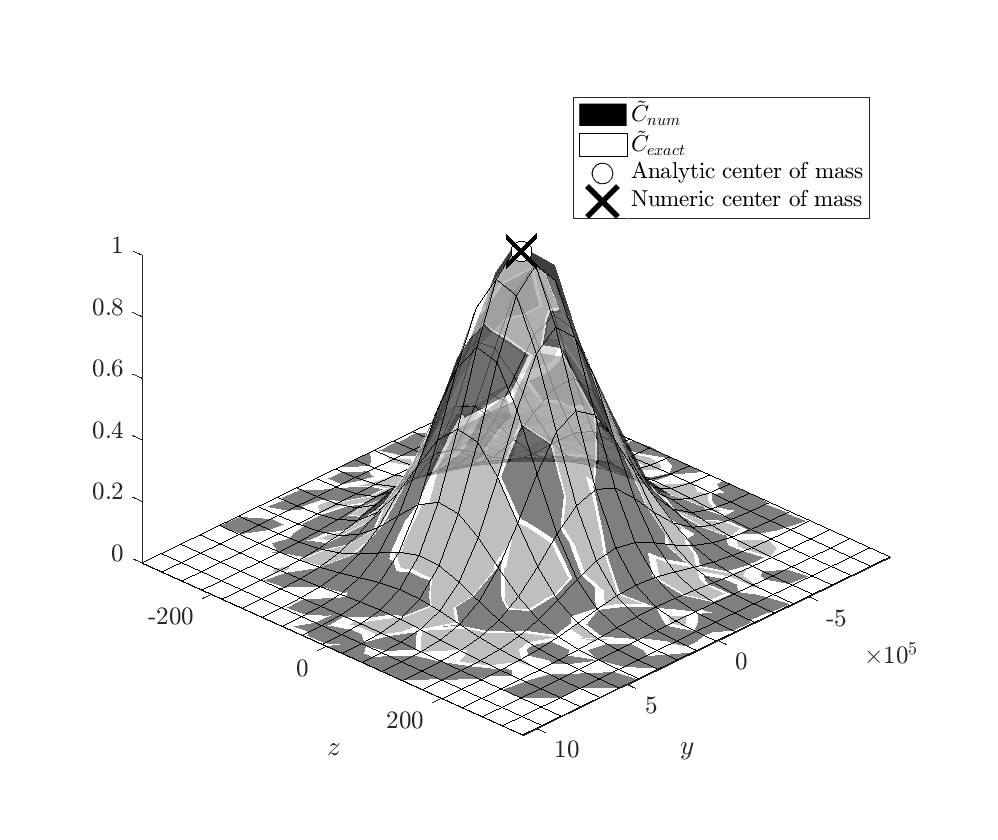
\includegraphics[width = \textwidth]{fig/testcase/testcase_surf.eps}
	\caption{Comparison of the concentrations obtained analytically and numerically. The "centers of mass" of the concentration obtained numerically (black cross) and numerically (white bullet) are also shown on the figure.}
	\label{fig:testcase_surf}
\end{figure}
\begin{figure}[H]
	\centering
	\begin{subfigure}[b]{0.49\textwidth}
		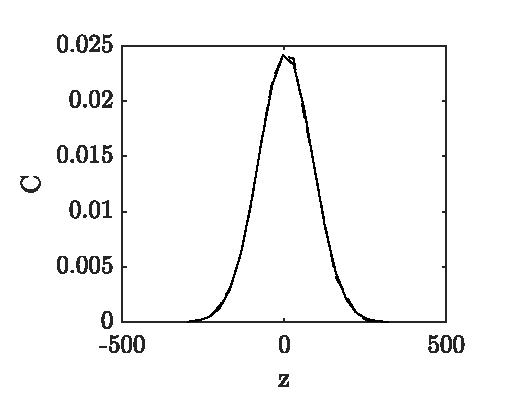
\includegraphics[width=\textwidth]{fig/testcase/testcase_fixedy.eps}
		\caption{$C_{num}(y_1+vT,z)$ and $C_{exact}(y_1+vT,z)$.}
		\label{fig:testcase_fixedy}
	\end{subfigure}
	\begin{subfigure}[b]{0.49\textwidth}
		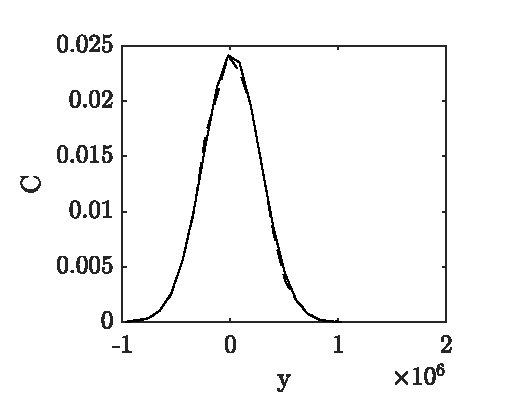
\includegraphics[width=\textwidth]{fig/testcase/testcase_fixedz.eps}
		\caption{$C_{num}(y,z_1+wT)$ and $C_{exact}(y,z_1+wT)$.}
		\label{fig:testcase_fixedz}
	\end{subfigure}
	\caption{Cut of the concentrations at fixed $y = r_{y,exact}$ and at fixed $z = r_{z,exact}$. The dashed line represent $C_{num}$ and the continuous line is for $C_{exact}$.}
\end{figure}

%-------------------------------------------RESULTS CASE 2-----------------------------------------------------------------------%
\subsection{Test case 2}
Figure \ref{fig:testcaseSI_surf} shows a comparison between the numerical result and the analytical solution for the (normalized) concentrations for test case 2. Since we do not have analytical expressions of the center of mass and of the variance for this test case, the "exact" values are approximated numerically thanks to the analytical expression of the concentration. Figures \ref{fig:testcaseSI_fixedy} and \ref{fig:testcaseSI_fixedz} represent respectively a cut of the concentrations at fixed $y = r_{y,exact}$ and along the boundary $z = 0$. The big picture about test case 2 is the presence of a boundary with no-through condition. A first verification is to check if all the particles are still in the domain, which is indeed the case. Although this might seem trivial here, it is sometimes a real challenge to ensure that no particle crosses the boundary, especially for geometrically complex domains. Besides, one can see on figure \ref{fig:testcaseSI_fixedz} that the concentration profile is well approximated along the boundary. Indeed, the maximal local error at the boundary is
\begin{equation}
	\|C_{exact}(y,0)-C_{num}(y,0)\|_{\infty} = 3.53\e{-4}, 
\end{equation}
The maximal local error on the whole domain is 
\begin{equation}
	\|C_{exact}-C_{num}\|_{\infty} = 1.097\e{-3}.
\end{equation}
The centers of mass are located at
\begin{equation}
	\b r_{exact} = (1.26\e{4},5.06\e{3}) \mbox{ [$m$],}\quad \b r_{num} = (1.10\e{4},5.05\e{3}) \mbox{ [$m$]}.
\end{equation}
The relative error is
\begin{equation}
	\b e_r = \left \lvert \frac{\b r_{exact}-\b r_{num}}{\b r_{exact}} \right \rvert =  \left(1.29\e{-1}, 1.825\e{-3}\right).
\end{equation}
The 2-norm of the relative error is
\begin{equation}
	\| \b e_r \|_2 = 1.29\e{-1}.
\end{equation}
This can be seen as a quantification of the error on advection. To quantify the error on diffusion, we compute the variance of the concentration :
\begin{equation}
	\sigma^2_{exact} = 6.39\e{10} \mbox{ [$m^2$],}\quad \sigma^2_{num} = 6.35\e{10} \mbox{ [$m^2$].}
\end{equation}
The relative error is
\begin{equation}
	e_{\sigma^2} = \left \lvert \frac{\sigma^2_{exact}-\sigma^2_{num}}{\sigma^2_{exact}}\right \rvert = 4.85\e{-3}.
\end{equation}
\begin{figure}[H]
	\centering
	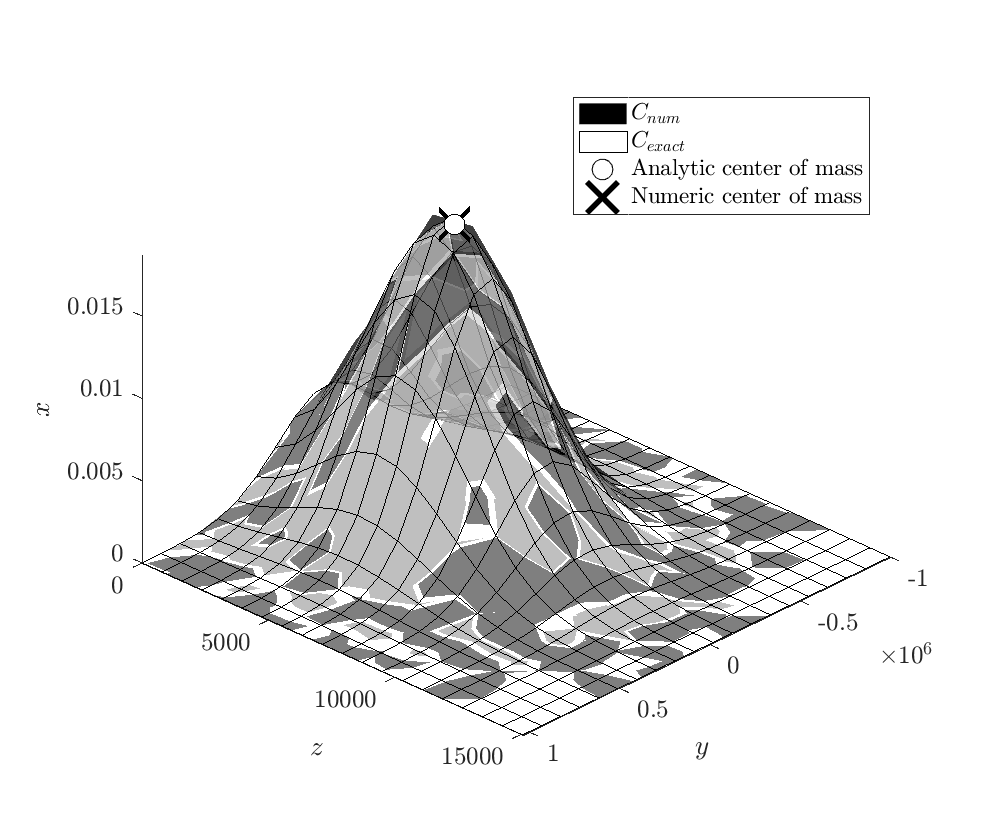
\includegraphics[width = \textwidth]{fig/testcase/testcaseSI_surf.eps}
	\caption{Comparison of the concentrations obtained analytically and numerically. The "centers of mass" of the concentration obtained numerically (black cross) and numerically (white bullet) are also shown on the figure.}
	\label{fig:testcaseSI_surf}
\end{figure}
\begin{figure}[H]
	\centering
	\begin{subfigure}[b]{0.49\textwidth}
		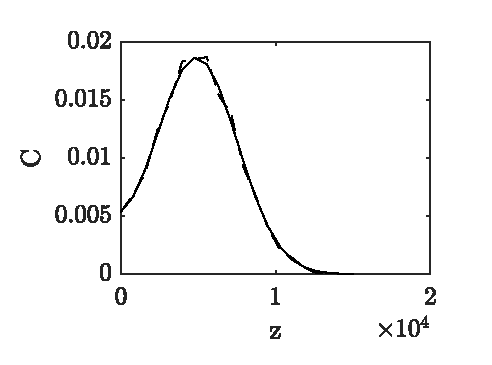
\includegraphics[width=\textwidth]{fig/testcase/testcaseSI_fixedy.eps}
		\caption{$C_{num}(y_1+vT,z)$ and $C_{exact}(y_1+vT,z)$.}
		\label{fig:testcaseSI_fixedy}
	\end{subfigure}
	\begin{subfigure}[b]{0.49\textwidth}
		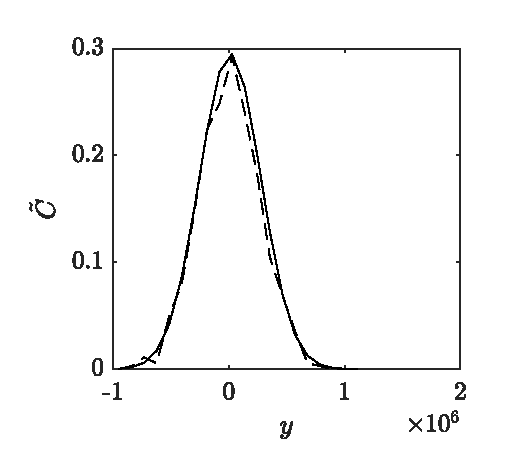
\includegraphics[width=\textwidth]{fig/testcase/testcaseSI_fixedz.eps}
		\caption{$C_{num}(y,z_1+wT)$ and $C_{exact}(y,z_1+wT)$.}
		\label{fig:testcaseSI_fixedz}
	\end{subfigure}
	\caption{Cut of the concentrations at fixed $y = r_{y,exact}$ and at fixed $z = r_{z,exact}$. The dashed line represent $C_{num}$ and the continuous line is for $C_{exact}$.}
\end{figure}